\chapter{Przegląd istniejących zbiorów}
Zbiory danych w kontekście uczenia maszynowego stanowią fundamentalny element wymagany do podejmowania wszelakich zadań. Mają one bardzo duży wpływ na skuteczność każdego modelu i z tego powodu przed przystąpieniem do tworzenia polskich wariantów zostało poświęcone wiele wysiłku na przeanalizowanie zbiorów istniejących.

Na początku bieżącego rozdziału dokładnie przedstawiony zostanie zbiór \code{Spider} ze szczególnym zwróceniem uwagi na jego format, którego należy przestrzegać podczas tworzenia wersji polskiej. W kolejnej części nastąpi przegląd zbiorów pokrewnych, czyli takich które powstały na fundamencie baz danych \code{Spider}. Jest to istotne, ponieważ część z nich również postanowiono przetłumaczyć na polski. Na koniec nastąpi dogłębna analiza istniejących tłumaczeń zbioru Spider, aby dokonać świadomych decyzji podczas tworzenia polskiego odpowiednika.

\section{Angielski Spider}
Spider to zbiór danych przeznaczony do zadania \code{Text-to-SQL}, składający się z 10181 próbek. Są one podzielone na część treningową, walidacyjną oraz testową. Cześć testowa nie jest jednak powszechnie dostępna. Ewaluowane są na niej modele wysyłane do publicznie dostępnego rankingu. Dzięki temu jest pewność, że dobre rezultaty modeli nie są skutkiem przypadkowego, ani celowego wycieku danych testowych do zbioru treningowego.

Próbki ze zbioru spider opierają się na 200 bazach danych. Są one bardzo różnorodne, ponieważ obejmują 138 domen. Bardzo ważne jest to, że są rozdzielone pomiędzy 3 części zbioru, co oznacza, że próbki w części testowej dotyczą baz danych, których w części treningowej nie mogło być. Wymusza to na tworzonych modelach posiadanie umiejętności uogólniania do nowych domen.

\subsection{Format zbioru}

Ze względu na unikatowość zbioru \code{Spider} wiele istniejących modeli go wykorzystuję i co za tym idzie, reprezentowany przez niego format stał się w pewien sposób standardem. Nie jest to prosty format tabelaryczny, jak to wygląda w postaci wielu zbiorów danych, lecz składają się na niego cztery jakościowo różne komponenty. Są to próbki same w sobie, poprawne zapytania SQL (ang. gold queries), schemat baz danych oraz same bazy. Nieco uproszczona struktura plików zbioru została zwizualizowana na rysunku \ref{fig:spider-structure} 

\begin{figure}[ht]
  \centering
    \begin{forest}
      for tree={
        inner sep=0pt,l=10pt,l sep=10pt,
        font=\ttfamily,
        grow'=0,
        child anchor=west,
        parent anchor=south,
        anchor=west,
        calign=first,
        edge path={
          \noexpand\path [draw, \forestoption{edge}]
          (!u.south west) +(7.5pt,0) |- node[fill,inner sep=1.25pt] {} (.child anchor)\forestoption{edge label};
        },
        before typesetting nodes={
          if n=1
            {insert before={[,phantom]}}
            {}
        },
        fit=band,
        before computing xy={l=15pt},
      }
    [Spider
      [database
        [db1]
        [db2]
        [...]
      ]
      [dev.json]
      [train\_spider.json]
      [train\_others.json]
      [dev\_gold.sql]
      [train\_gold.sql]
      [tables.json]
    ]
    \end{forest}
\caption{Struktura plików zbioru \code{Spider}}
  \label{fig:spider-structure}
\end{figure}

\subsubsection{Próbki (\code{dev.json}, \code{train\_spider.json}, \code{train\_others.json})} 
Próbki przechowywane są w formacie json i podzielone zostały na trzy pliki. W pliki \code{dev.json} znajdują się próbki odpowiadające zbiorowi walidacyjnemu, natomiast w plikach \code{train\_spider.json} oraz \code{train\_others.json} umieszczono próbki treningowe. Są one rozdzielone dodatkowo na dwa pliki, ponieważ w pierwszym twórcy zbioru umieścili swoje autorskie próbki, natomiast w drugim próbki wyselekcjonowane z już istniejących zbiorów. Przykładowa próbka została przedstawiona na listingu \ref{lst:spider-sample}.

\begin{minipage}{\linewidth}
\lstinputlisting[
caption=Przykładowa próbka ze zbioru Spider z pliku \code{dev.json}, label={lst:spider-sample}, language=json
]{listings/spider_sample.json}
\end{minipage}

Znaczenie poszczególnych atrybutów próbki jest następujące:
\begin{itemize}
    \item \textbf{\code{db\_id}} - Identyfikator bazy danych, której próbka dotyczy.
    \item \textbf{\code{question}} - Pytanie w języku naturalnym.
    \item \textbf{\code{question\_toks}} - Pytanie podzielone na tokeny .
    \item \textbf{\code{query}} - Zapytanie SQL.
    \item \textbf{\code{query\_toks}} - Zapytanie SQL podzielone na tokeny.
    \item \textbf{\code{query\_toks\_no\_value}} - Zapytanie SQL podzielone na tokeny, ale z zamaskowanymi wszystkimi wartościami, a dokładnie zastąpionymi tekstem \code{"value"}.
    \item \textbf{\code{sql}} - Skomplikowany obiekt JSON będący sparsowanym zapytaniem SQL, pozwalający na szybkie liczenie metryk i umożliwiający łatwe wydobywanie różnych fragmentów zapytania.
\end{itemize}

\subsubsection{Poprawne zapytania SQL (\code{dev\_gold.sql}, \code{train\_gold.sql})}
Poprawne zapytania SQL zgodnie z powyższym opisem stanowią jeden z atrybutów próbek, lecz poza tym są one wyciągnięte do dwóch osobnych plików \code{dev\_gold.sql} oraz \code{train\_gold.sql}, które odpowiadają części walidacyjnej oraz treningowej. W każdej linii w tych plikach, jak przedstawiono na listingu \ref{lst:spider-gold}, umieszczone jest zapytanie SQL oraz nazwa bazy danych oddzielone od siebie za pomocą znaku tabulacji.

\begin{minipage}{\linewidth}
\lstinputlisting[
caption=Fragment pliku \code{dev\_gold.json} zawierającego poprawne zapytania SQL, label={lst:spider-gold}, language=SQL
]{listings/spider_gold.txt}
\end{minipage}

\subsubsection{Schemat (\code{tables.json})}
Plik \code{tables.json}, którego fragment został przedstawiony na listingu \ref{lst:spider-tables}, opisuję strukturę każdej zawartej w zbiorze Spider bazy danych. Obejmuję to nazwy wszystkich tabel i kolumn, typy kolumn, wskazane są kolumny stanowiące klucze podstawowe oraz obce.

Co ciekawe, oprócz oryginalnie występujących w bazie nazw tabel i kolumn w pliku schematu znajdują się również ich odpowiedniki w języku naturalnym. Oznacza to, że nazwy składające się z kilku słów i zapisywane oryginalnie za pomocą różnych konwencji, takich jak Camel Case, Snake Case, czy Pascal Case, są zamieniane na naturalną postać słów odseparowanych spacjami. Poza tym, część oryginalnych, skrótowych nazw jest rozwijana do zrozumiałej postaci. Jest to dodatkowa informacja, która nie jest dostępna w większości baz danych, a mimo wszystko jest wykorzystywana przez wiele algorytmów.

\lstinputlisting[
float, caption=Fragment pliku \code{tables.json} opisujący schemat pojedynczej bazy danych, label={lst:spider-tables}, language=json
]{listings/spider_tables.json}

\subsubsection{Bazy danych (\code{database/*})}
Ostatnim komponentem zbioru Spider jest katalog \code{database} zwierający szereg podkatalogów o nazwach odpowiadających identyfikatorom baz danych. Wewnątrz każdego z tych podkatalogów umieszczona jest baza danych SQLite oraz opcjonalnie dodatkowe pliki, takie jak skrypt SQL pozwalający zbudować daną bazę od zera. Większość baz, z nielicznymi wyjątkami, jest wypełniona danymi. Jest to istotne, ponieważ duża część nowoczesnych algorytmów opiera się na tych danych, by generowane zapytania SQL były dokładniejsze.

% \begin{figure}[ht]
%   \centering
%     \begin{forest}
%       for tree={
%         inner sep=2pt,l=10pt,l sep=10pt,
%         font=\ttfamily,
%         grow'=0,
%         child anchor=west,
%         parent anchor=south,
%         anchor=west,
%         calign=first,
%         edge path={
%           \noexpand\path [draw, \forestoption{edge}]
%           (!u.south west) +(7.5pt,0) |- node[fill,inner sep=1.25pt] {} (.child anchor)\forestoption{edge label};
%         },
%         before typesetting nodes={
%           if n=1
%             {insert before={[,phantom]}}
%             {}
%         },
%         fit=band,
%         before computing xy={l=15pt},
%       }[database
%         [world\_1
%             [world\_1.sqlite]
%             [world\_1.sql]
%         ]
%         [wrestler
%             [wrestler.sqlite]
%             [schema.sql]
%         ]
%         [...]
%       ]
%     \end{forest}
% \caption{Struktura katalogu Database zbioru Spider}
%   \label{fig:crontab}
% \end{figure}


\section{Angielskie zbiory pokrewne} \label{text:related-datasets}
Jedną z ważniejszych zasług zbioru Spider było zgromadzenie pokaźnej liczby baz danych pochodzących z bardzo różnych domen. Było to trudne ponieważ stanowią one informacje poufne dla wykorzystujących je firm i niewielka ich liczba jest dostępna w internecie. Nic więc dziwnego, że na fundamencie baz danych \code{Spider} powstało kilka nowych zbiorów. Doskonałym tego przykładem są zbiory \code{CoSQL} oraz \code{SParC}, gdzie zachowano te same bazy danych, lecz stworzone zostały całkowicie nowe przykłady. Pojawiło się również odmienne podejście polegające na stworzeniu nowych zbiorów poprzez dokonanie w próbkach ze zbioru Spider pewnych ukierunkowanych modyfikacji, czego przykładem są zbiory \code{Spider-Syn}, \code{Spider-DK} oraz \code{Dr.Spider}.

Jako, że część ze wspomnianych powyżej zbiorów pokrewnych do zbioru \code{Spider} odegrało istotną rolę w procesie tworzenia polskiego zbioru danych, to zostaną one pobieżnie opisane w poniższych podsekcjach.

\subsection{Spider-Syn}
\code{Spider-Syn} jest zbiorem danych powstałym ze zbioru \code{Spider} poprzez zmodyfikowanie próbek w taki sposób, aby ograniczyć dosłowne wymienianie w pytaniach nazw kolumn, tabel i wartości z bazy. Odzwierciedla to scenariusz w którym z interfejsu tekstowego do bazy korzysta osoba, która dokładnie jej nie zna, więc często posługuję się synonimami. Stworzenie tego typu zbioru było istotne, ponieważ okazało się, że duża część istniejących algorytmów opiera się na powiązywaniu pytania z elementami bazy poprzez znajdywanie dosłownych powtórzeń i w przedstawionym scenariuszu ich skuteczność radykalnie spada. Zmodyfikowana została jednak jedynie nieco ponad połowa próbek, ponieważ dla dużej części przykładów ciężkim było znalezienie odpowiednich synonimów.

\begin{minipage}{\linewidth}
\lstinputlisting[
caption=Przykład próbki ze zbioru \code{Spider-Syn}, label={lst:spider-syn-example}, language=json
]{listings/spider_syn_example.json}
\end{minipage}

\subsection{Spider-DK}
Zbiór danych \code{Spider-DK} (skrót od Domain Knowledge) został zbudowany w oparciu o zbiór testowy \code{Spider} w celu oceny uogólniania modeli \code{Text-to-SQL}, ze szczególnym uwzględnieniem rozumienia wiedzy dziedzinowej. \code{Spider-DK} zawiera 535 par pytań w języku naturalnym i zapytań SQL, z czego 270 par jest identycznych jak w oryginalnym Spiderze, a pozostałe 265 par zostało zmodyfikowanych tak, aby uwzględnić wiedzę dziedzinową. Pytania w \code{Spider-DK} wymagają zrozumienia 5 typów wiedzy dziedzinowej: pomijanie wymieniania kolumn, proste wnioskowanie, synonimy wartości komórek, generowanie warunków na podstawie słów spoza wartości komórek oraz wiedza, która łatwo kłóci się z innymi dziedzinami. \code{Spider-DK} symuluje scenariusz, w którym w zapytaniu użytkownika wykorzystywana jest konkretna wiedza dziedzinowa.

\begin{minipage}{\linewidth}
\lstinputlisting[
caption=Przykład próbki ze zbioru \code{Spider-DK}, label={lst:spider-dk-example}, language=json
]{listings/spider_dk_example.json}
\end{minipage}

\subsection{SParC}
\code{SParC} jest zbiorem danych zawierającym sekwencje pytań w języku naturalnym oraz odpowiadające im zapytania SQL. Zbiór zawiera 4298 spójnych sekwencji pytań (łącznie ponad 12 tysięcy pojedynczych pytań), dotyczących baz danych \code{Spider}. Został stworzony przez 15 studentów posiadających doświadczenie w SQL. Pytania są tematycznie powiązane i wymagają wykorzystania informacji z poprzednich pytań, aby poprawnie sformułować odpowiednie zapytanie SQL.

\begin{figure}[ht!]
  \centering
  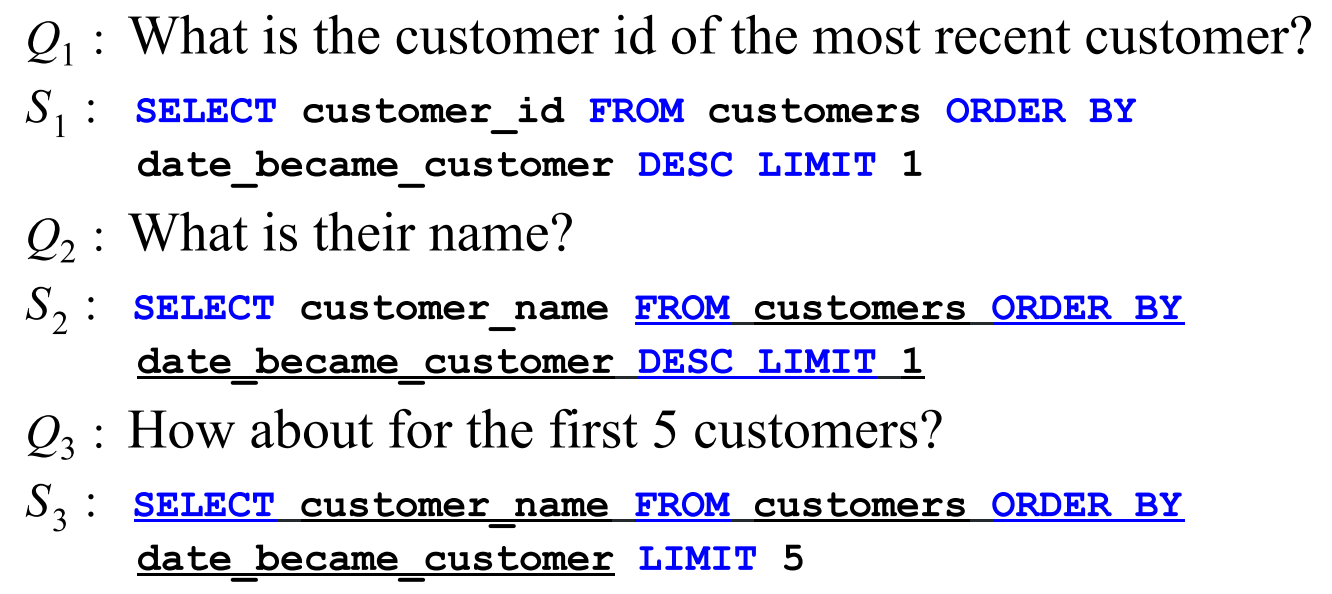
\includegraphics[width=0.6\linewidth]{images/sparc_example.png}
  \caption{Przykładowa konwersacja ze zbioru \code{SParC}}
  \label{fig:sparc-example}
\end{figure}

\subsection{CoSQL}
\code{CoSQL} to pierwszy duży korpus tekstowych zapytań SQL zebranych w konwersacyjnej formie. Zawiera on ponad 30 000 fragmentów dialogów oraz ponad 10 000 adnotowanych zapytań SQL, pozyskanych w ramach symulowanych rozmów pomiędzy zwykłymi użytkownikami a ekspertami SQL na temat baz danych i domen pochodzących oryginalnie ze zbioru \code{Spider}. Każdy dialog odtwarza realistyczny scenariusz eksploracji bazy danych, w którym użytkownik zadaje pytania, a ekspert SQL stara się na nie odpowiedzieć, wyjaśniając niejednoznaczne kwestie lub informując o pytaniach bez odpowiedzi. Gdy pytania użytkownika dają się sformułować w języku SQL, ekspert opisuje je w tym języku i prezentuje wyniki, aby zachować naturalny przebieg interakcji.

\begin{figure}[ht!]
  \centering
  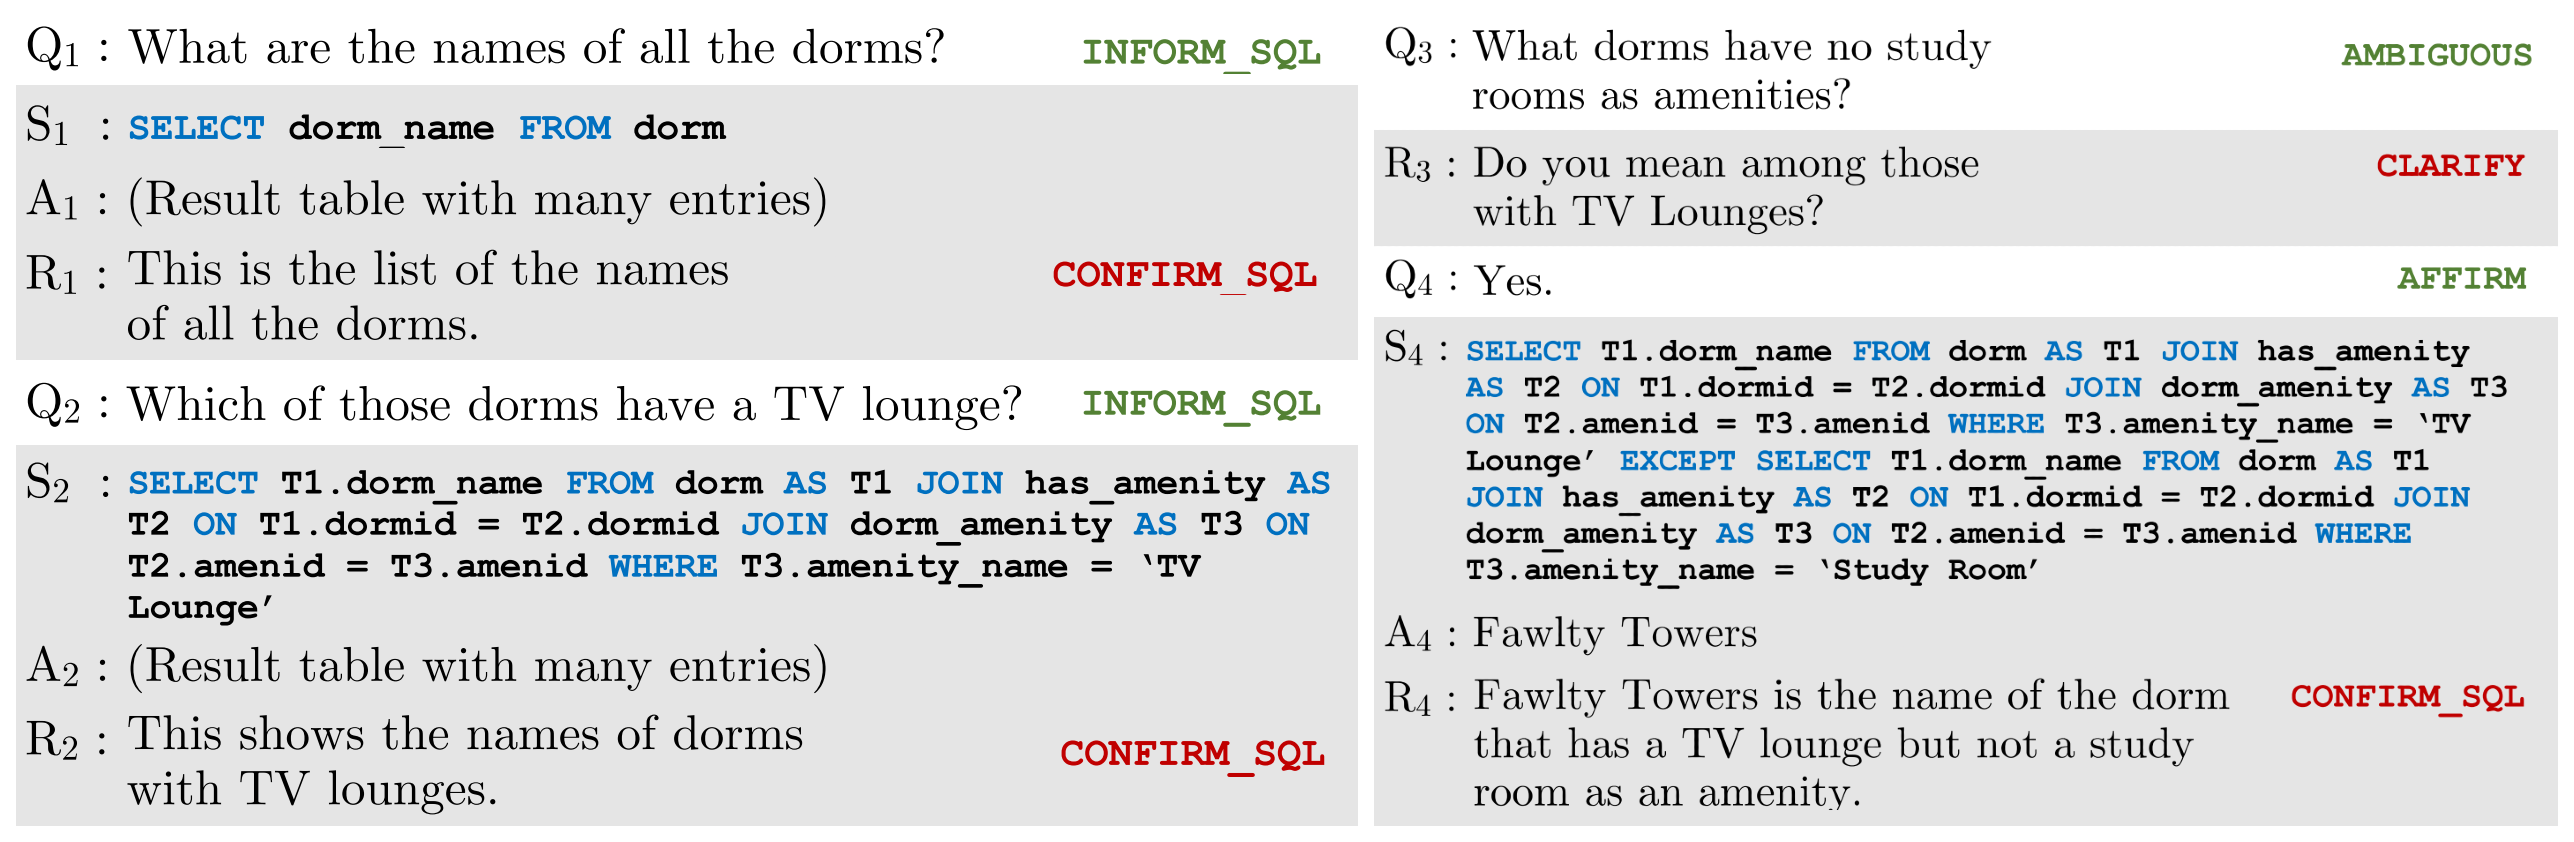
\includegraphics[width=1.0\linewidth]{images/cosql_example.png}
  \caption{Przykładowa konwersacja ze zbioru \code{CoSQL}}
  \label{fig:cosql-example}
\end{figure}

\section{Istniejące tłumaczenia zbioru Spider}
Jak zostało wspomniane podczas przeglądu literatury, obecnie istnieją cztery tłumaczenia zbioru Spider na języki narodowe. Jest to język chiński, wietnamski, portugalski oraz rosyjski. Autorzy tych zbiorów jednak pomimo wspólnego celu podeszli do zadania na różne sposoby. Celem niniejszej sekcji jest przedyskutowanie kluczowych różnic pomiędzy nimi. Jedną z najistotniejszych jest zastosowana metoda tłumaczenia. Rozbieżności zaobserwowano również jeśli chodzi o tłumaczenie schematu, zawartość baz danych oraz wartości w zapytaniach. Różnice w tych kwestiach zostały zestawione w tabeli \ref{tab:spider-trans-diffs} i zostaną dogłębnie omówione w poniższych sekcjach.


\begin{table}[ht]
    \centering
    \begin{tabular}{|l|c|c|c|c|}
        \hline
        \thead{Zbiór} & 
        \thead{Rodzaj\\tłumaczenia} &
        \thead{Tłumaczenie\\schematu} &
        \thead{Tłumaczenie\\zawartości\\baz danych} &
        \thead{Tłumaczenie\\wartości w\\zapytaniach} \\
        \hline
        \makecell{Chiński\\(\code{CSpider})} & Manualne & Nie & Nie & Tak \\
        \hline
        \makecell{Wietnamski\\(\code{ViText2SQL})} & Manualne & Tak & Nie & Tak \\
        \hline
        \makecell{Portugalski} & Maszynowe & Tak & Nie & Nie \\
        \hline
        \makecell{Rosyjski\\(\code{PAUQ})} & Manualne & Nie & Częściowo & Tak \\
        \hline
    \end{tabular}
    \caption{Zestawienie kluczowych różnic pomiędzy tłumaczeniami zbioru \code{Spider}}
    \label{tab:spider-trans-diffs}
\end{table}

\subsection{Rodzaj tłumaczenia} \label{text:translation-method}
Tłumaczenie maszynowe i manualne to dwa możliwe podejścia. Pierwsze sprowadza się do wykorzystania narzędzi, dostępnych najczęściej za pomocą webowych API, takich jak \code{Google Cloud Translation API} \cite{google-translation-api}, czy \code{DeepL} \cite{deepl}. Drugie natomiast oznacza ręczne tłumaczenie każdej próbki przez człowieka. Oczywiście tłumaczenie ręczne może być wspomagane przez metodę maszynową, aby ograniczyć się do poprawiania tłumaczeń zamiast pisania ich od początku.

Największą zaletą tłumaczenia maszynowego jest szybkie uzyskanie przetłumaczonego zbioru. Wiąże się to najczęściej z naliczeniem pewnych kosztów, o których trzeba wspomnieć, lecz mimo wszystko koszt ten jest niewspółmierny do ceny wynajęcia profesjonalnego ludzkiego tłumacza. Jest on również pomijalny w stosunku do czasu, który trzeba by poświęcić, by dokonać tłumaczenia samemu.

Tłumaczenie maszynowe ma jednak istotne wady - dostępne narzędzia stają się coraz lepsze, lecz jednak wciąż nie dorównują człowiekowi. Sprawia to, że uzyskiwane zbiory danych są bezsprzecznie niższej jakości. Narzędzia te dokonując tłumaczenia zbioru Spider nie biorą pod uwagę wielu istotnych elementów, które ludzki adnotator by uwzględnił. Przykładem jest ignorowanie domeny podczas tłumaczenia pytania naturalnego. Ludzki tłumacz pytanie \enquote{list all parties} w domenie politycznej przetłumaczy jako \enquote{zwróć wszystkie partie}, natomiast tłumacz maszynowy przetłumaczy to bez wątpienia jako \enquote{zwróć wszystkie imprezy}.

Dotychczasowe tłumaczenia zbioru Spider, z powodu ograniczeń metody maszynowej, w większości korzystają z ręcznego tłumaczenia zbioru. Jest to prawdą dla rosyjskiego \code{PAUQ}, wietnamskiego \code{ViText2SQL} oraz chińskiego \code{CSpider}, jedyny wyjątek stanowi zbiór portugalski. Autorzy każdego z tych manualnie tłumaczonych zbiorów dla porównania dokonali również tłumaczenia maszynowego. Zestawienie wyników osiąganych przez modele trenowane na zbiorach tłumaczonych maszynowo i manualnie zostało przedstawione w tabeli \ref{tab:manual-vs-machine}. Wszystkie wyniki potwierdzają, że tłumaczenie manualne pozwala uzyskać lepsze wyniki, aczkolwiek w przypadku względnie nowych modeli \code{RAT-SQL} oraz \code{BRIDGE} procentowy spadek skuteczności na zbiorach maszynowych nie jest tak znaczący jak dla modeli wcześniejszych.

\begin{table}[ht]
    \centering
    \begin{tabular}{|c|c|c|c|c|}
        \hline
        \thead{Zbiór} & \thead{Model} & \thead{Maszynowe} & \thead{Manualne} &
        \thead{Różnica} \\
        \hline
        CSpider & C-ML & \s7,9 & 12,1 & \s4,1 \\
        \hline
        CSpider & W-ML & \s0,6 & 10,0 & \s2,4 \\
        \hline
        ViText2SQL & EditSQL (Vi-Syllable) & 16,8 & 24,1 & \s7,3 \\
        \hline
        ViText2SQL & EditSQL (Vi-Word) & 17,4 & 30,2 & 12,8 \\
        \hline
        PAUQ & RAT-SQL & 46,0 & 51,0 & \s5,0 \\
        \hline
        PAUQ & BRIDGE & 49,0 & 52,0 & \s3,0 \\
        \hline
    \end{tabular}
    \caption{Zestawienie wyników metryki exact match na części testowej dla tłumaczeń maszynowych i manualnych.}
    \label{tab:manual-vs-machine}
\end{table}

\subsection{Tłumaczenie schematu}
Kolejną kwestią dokonującą podziału wśród istniejących tłumaczeń zbioru \code{Spider} jest obrane podejście co do wynikowego języka schematu baz danych, czyli nazw tabel i kolumn - mogą być one tłumaczone lub pozostawione bez zmian w języku angielskim. To drugie podejście jest uzasadnione faktem, że w praktyce, niezależnie od kraju, schemat baz danych jest często utrzymywany w języku angielskim. Ma takie zalety jak ułatwienie pracy wielonarodowemu zespołowi, czy też uniknięcie problemu ze znakami diakrytycznymi, których wykorzystywanie może być niemożliwe lub utrudnione.

Fakt, że w praktyce nazwy tabel i kolumn są zapisywane w języku angielskim w swoich artykułach podkreślili autorzy tłumaczenia chińskiego oraz rosyjskiego i z uwagi na to postanowili schematu baz nie tłumaczyć. Twórcy zbioru wietnamskiego i portugalskiego postanowili jednak tłumaczenia dokonać, nie przedstawiając dla tego żadnego uzasadnienia.

Należy zwrócić uwagę, że reprezentowanie pytań i schematu baz danych w dwóch różnych językach znacząco komplikuję rozwiązywany problem. W wersji, gdy wszystkie komponenty są w tym samym języku to dość łatwo jest znaleźć powiązania pomiędzy nimi, ponieważ wystarczy przeanalizować ich podobieństwo jako łańcuchów znaków. W innym przypadku to jednak nie wystarczy - wykorzystywany model musi posiadać dodatkowo pewne cechy tłumacza.

Podsumowując, pozostawienie schematu bazy danych w języku oryginalnym jest uzasadnione z praktycznego punktu widzenia, jednak dodatkowo komplikuje zadanie. Zbiór danych z przetłumaczonym schematem, chociaż pomija aspekt praktyczny, stanowi lepszy odpowiednik oryginalnego Spidera i pozwala na wykonywanie względem niego sprawiedliwych porównań.

\subsection{Tłumaczenie zawartości baz danych}
Kolejną niespójnością jaką można zaobserwować pomiędzy istniejącymi tłumaczeniami zbioru \code{Spider} jest kwestia tłumaczenia zawartości baz danych. Dokonanie takiego tłumaczenia ma istotne zalety przedstawione w kolejnych akapitach, jednak jest to zadanie problematyczne, przez co nie wszyscy autorzy zbiorów się go podjęli.

Większość nowych podejść do problemu generowania SQL analizuje znajdujące się w bazach danych rekordy, aby zwiększyć swoją skuteczność. Przykładowo użytkownik systemu może poprosić o zwrócenie populacji Polski, a dwie możliwe odpowiedzi mogłyby zawierać fragmenty \sql{WHERE country = 'PL'} oraz \sql{WHERE country = 'polska'}. Widać tutaj, że schemat bazy nie mówi wszystkiego i bez dostępu do jej zawartości obie odpowiedzi są równie dobre, choć tylko jedna poprawna. W celu wytrenowania najlepszych modeli przygotowany zbiór powinien zawierać wypełnione bazy danych, a większość istniejących modeli korzystających z zwartości bazy, zakłada, że jest ona w tym samym języku co pytania.

Drugim zastosowaniem wartości w bazach danych jest umożliwienie ewaluacji przygotowanych algorytmów przy pomocy metryki execution accuracy. Została ona opisana dokładnie w dalszej części pracy w sekcji x.xx. Jej skrótowa zasada działania polega na wykonaniu prawidłowych zapytań oraz zapytań wygenerowanych i uznaniu poprawnymi tych, które zwróciły te same wyniki. Przetłumaczenie wartości w zapytaniach SQL bez tłumaczenia zawartości baz danych skutkuję tym, że wykonywane zapytania często nie zwracają żadnych wyników, a co za tym idzie, wiele nieprawidłowo wygenerowanych zapytań jest uznawanych omyłkowo za prawidłowe. Podsumowując, różne języki wartości w zapytaniach SQL i wartości w bazach danych skutkują upośledzeniem metryki execution accuracy i zmniejszeniem jej użyteczności.

Wśród przedstawionych wersji zbioru \code{Spider} modyfikacji zawartości bazy danych podjęli się jedynie autorzy tłumaczenia rosyjskiego. Nie tłumaczyli oni jednak wszystkich wartości, ale tylko te, które wystąpiły w przynajmniej jednym zapytaniu. Powodem dla którego pozostałe zbiory obyły się bez tłumaczenia zapewne jest duża liczba danych zawartych w bazach i relatywnie niewielkie korzyści wynikające z ich tłumaczenia. Autorzy zbioru portugalskiego rozwiązali ten problem w jeszcze inny sposób - postanowili nie tłumaczyć wartości w zapytaniach, dzięki czemu znajdujące się w nich wartości i w bazach danych były w tym samym języku. Takie podejście wydaje się jednak naciągane, bo mało praktyczne - zakłada scenariusz w których w bazach danych o portugalskim schemacie przechowywane są wartości angielskie.
